\chapter{Globally hyperbolic spacetimes}\label{chapter:4}

From now on we will only work with Lorentzian manifolds of dimension $(2+1)$.\\
The aim of this section is to classify maximal globally hyperbolic spacetimes with compact Cauchy surface of genus $n\geq 2$. To do so, we have to study causal properties of Anti-de Sitter geometry and isometric actions, which constitute the fundamental setup for the proofs of Mess' classification results.\\
Here we will first study achronal sets in the conformal compactification of Anti-de Sitter space, a notion that makes sense in the universal cover $\AS^{2,1}$, and then adapt the notion
for subsets of $\A^{2,1}$. We will also introduce the fundamental notions of invisible domain and of domain of dependence, and describe their properties.

\section{Achronal and acausal set}
\begin{definition}
    A subset $X \subset \AS^{2,1} \cup \partial\AS^{2,1}$ is \textit{achronal} (resp. \textit{acausal}) if no pair of points in $X$ are connected by timelike (resp. causal) lines in $\AS^{2,1}$
\end{definition}
Consider the Poincaré model $\D\times\R$ of $\AS^{2,1}$ equipped with the hemispherical metric $g_{\mathbb{S}^2} - dt^2$ introduced in Section \ref{sec:geodesic}. The following lemma gives a charecterization of achronal/acausal set:
\begin{lemma}\label{lem:1-lip}
    A subset $X$ of $\AS^{2,1} \cup \partial\AS^{2,1}$ is achronal (resp. acausal) if and only if it is the graph of a function $f : D \to \R$ that is 1-Lipschitz (resp. strictly 1-Lipschitz) with respect to the distance induced by the hemispherical metric $g_{\mathbb{S}^2}$. Here $D$ denotes the projection of $X$ to the $\D$ factor.
\end{lemma} 
\begin{proof}
    Assume that $X$ is an achronal set. The restriction of the projection $\pi_\D : \D \times \R \to \D$ to $X$ is injective, since vertical lines in the Poincaré model are timelike. So $X$ can be regarded as the graph of a function $f : D \to\R$. Imposing that $(x,f(x))$ and $(y,f(y))$ are not related by a timelike curve we can deduce that
    \begin{equation} \label{eq:achronal}
        |f(x) - f(y)| \leq d_{\mathcal{S}^2}(x,y),
    \end{equation}
    where $d_{\mathcal{S}^2}$ is the hemispherical distance. The same argument shows that the graph of a 1-Lipschitz function defined on some subset of $\D$ is achronal.\\
    Moreover, two points $(x,t)$ and $(y,s)$ are on the same lightlike geodesic if and only if $|t-s| =  d_{\mathcal{S}^2}(x,y)$. Therefore $X$ is acausal if and only if the inequality in (\ref{eq:achronal}) is strict.
\end{proof}
A 1-Lipschitz function on a region $D \subset \D$ extends uniquely to the boundary of $D$. As a consequence of the previous lemma we have:
\begin{lemma}\label{lem:global 1-lip}
    An achronal subset $X$ in $\A^{2,1}$ is properly embedded if and only if it is a global graph over $\D$. In this case it extends uniquely to the graph of a 1-Lipschitz function over $\D \cup \partial \D$.
\end{lemma}
In the following, we refer to an achronal subset $X$ in $\A^{2,1}$ which is the graph of a 1-Lipschitz function defined on a domain of $\D$ as an \textit{achronal surface}. Recall the following definition
\begin{definition}
    Given a surface $S$ and a Lorentzian manifold $(M,g)$, a $C^1$ immersion $\sigma : S \to M$ is \textit{spacelike} if the pull-back metric $\sigma^* g$ is a Riemannian metric. In this setting $\sigma(S)$ is said to be a \textit{spacelike surface}.
\end{definition}
A spacelike surface is locally acausal, but there are examples of spacelike surfaces which are not even achronal. A spacelike surface is acausal when it is properly embedded in $\AS^{2,1}$. 
\begin{lemma}\label{lem:lightlike}
    Let $S$ be a properly embedded achronal surface of $\AS^{2,1} \cup \partial\AS^{2,1}$. If a lightlike geodesic segment $\gamma$ joins two points of $S$ then $\gamma$ is contained in $S$.
\end{lemma}
\begin{proof}
    Let $f^S:\overline{\D} \to \R$ be the function 1-Lipschitz defining $S$. If $\gamma$ joins $(x,f^S(x))$ and $(y,f^S(y))$ then (up to switching the role of $x$ and $y$) $f^S(y) = f^S(x) + d_{\mathcal{S}^2}(x,y)$. Moreover, $\gamma$ consists of points of the form $(z,f^S(x) + d_{\mathcal{S}^2}(x,z))$, for $z$ lying on the $g_{\mathcal{S}^2}$-geodesic segment joining $x$ to $y$. By achronality of $S$ we have
    \[
        f^S(z) - f^S(x) \leq d_{\mathcal{S}^2}(x,z)
    \]
    and 
    \[
        f^S(x) - f^S(z) \leq d_{\mathcal{S}^2}(z,y) = d_{\mathcal{S}^2}(x,y) - d_{\mathcal{S}^2}(x,z),
    \]
    which implies that $f^S(z) \geq f^S(x) + d_{\mathcal{S}^2}(x,z)$. Therefore we can conclude $f^S(z) = f^S(x) + d_{\mathcal{S}^2}(x,z)$, proving that $\gamma$ is contained in $S$.
\end{proof}
Given a function $f: \overline{\D}\to\R$, we define its oscillation as 
\[
    osc(f):= \max_{y\in\overline{\D}} f(y) - \min_{y\in\overline{\D}} f(y).
\]
\begin{lemma}\label{lem:osc}
    Let $S$ be a properly embedded achronal surface, defined as the graph of $f^S:\overline{\D} \to \R$, then $osc(f^S) \leq \pi$. Moreover $osc(f^S)= \pi$ if and only if $S$ is a lightlike plane.
\end{lemma}
\begin{proof}
    As $f^S$ is 1-Lipschitz and the diameter of $\D$ for $g_{\mathcal{S}^2}$ is $\pi$, then $osc(f^S)$ is bounded by $\pi$. Moreover, if $osc(f^S)=\pi$ then there are two antipodal points $y,y'\in \partial \D$ such that $f^S(y')=f^S(y) + \pi$. Recall that the lightlike plane with past and future points $(y,f^S(y))$ and $(y',f^S(y)+\pi)$ is
    \[
        P = \{ (x,t) \ | \ t=f^S(y) + d_{\mathcal{S}^2}(x,y) \}
    \]
    and it is foliated by lightlike geodesics joining $(y,f^S(y))$ to $(y',f^S(y)+\pi)$. By Lemma \ref{lem:lightlike}, $P$ is included in $S$. Since $P$ and $S$ are both global graphs over $\overline{\D}$, $S=P$.
\end{proof}
    


\section{Invisible domain}
\begin{definition}
    Let $X$ be an achronal set in $\AS^{2,1} \cup \partial\AS^{2,1}$, the \textit{invisible domain} of $X$ is the subset $\Omega(X) \subset \AS^{2,1}$ of points which are connected to $X$ by no causal path.
\end{definition}
By a result of McShane \cite{mcshane1934extension} any 1-Lipschitz function on a subset of a metric space admits a 1-Lipschitz extension everywhere. Hence any achronal set is a subset of a properly embedded achronal surface.
Given an achronal set $X$ defined as $f^X : D \to \R$ there are two particular extensions called \textit{extremal extensions}:
\[
\begin{array}{cc}
    f_-^X(y)= \sup_{x\in D}\{ f^X(x)-d_{\mathcal{S}^2}(x,y) \}, & f_+^X(y)= \inf_{x\in D}\{ f^X(x)+d_{\mathcal{S}^2}(x,y) \}
\end{array}
\]
\begin{lemma}\label{lem:extremal extension}
    Let $X$ be a closed achronal subset of $\AS^{2,1} \cup \partial\AS^{2,1}$ and let $S_\pm (X)$ be the graphs of the extremal extensions $f^X_\pm$:
    \begin{itemize}
        \item The properly embedded surfaces $S_-(X)$ and $S_+(X)$ are achronal with $S_\pm(X) \subset \overline{\text{I}^\pm (S_\mp(X))}$, and $\Omega(X) = \text{I}^+(S_-(X)) \cap \text{I}^-(S_+(X))$.
        \item Every achronal subset containing $X$ is contained in $S_-(X)\cup\Omega(X)\cup S_+(X)$.
        \item Every point in $S_\pm(X)$ is connected to $X$ by at least one lightlike geodesic segment which is entirely contained in $S_\pm(X)$. Moreover $S_+(X) \cap S_-(X)$ is the union of $X$ and all lightlike geodesic segments joining points of $X$.
    \end{itemize}
\end{lemma}

\begin{observation}\label{rem:invisible}
    $S_-(X)\cup\Omega(X)\cup S_+(X)$ is the set of points connected to any point of $X$ by spacelike or lightlike geodesic. In particular $\Omega(X)$ consists of points connected to any point of X by a spacelike geodesic.
\end{observation}
\begin{observation}
    The intersection of any properly embedded achronal surface containing
    $X$ with $S_\pm(X)$ is a union of lightlike geodesic segments with an endpoint in $X$. In particular any properly embedded acausal surface containing $X$ is contained in the region $\Omega(X)$.
\end{observation}

\section{Achronal meridians}
\begin{definition}
    An \textit{achronal meridian} in $\AS^{2,1}$ is a subset $\Lambda$ of $\partial\AS^{2,1}$ that is the graph of a 1-Lipschitz function $f: \partial\D\to\R$.
\end{definition}
The importance of these definitions will be evident in the following sections.
The invisible domain of a achronal meridian will be a fundamental tool in the study of globally hyperbolic spacetimes.
\begin{lemma}
    Let $\Lambda$ be an achronal meridian in $\partial\AS^{2,1}$ different from the boundary of a lightlike plane. Then $S_+(\Lambda) \cap S_-(\Lambda)=\Lambda$. Moreover there is an achronal properly embedded surface in $\Omega(\Lambda)$ whose boundary in $\partial\AS^{2,1}$ is $\Lambda$.
\end{lemma}
\begin{proof}
    By Lemma \ref{lem:osc} the maximal oscillation of $f:\partial\D \to \R$ that defines $\Lambda$ is smaller than $\pi$. If a lightlike geodesic connects $(x,f(x))$ to $(y,f(y))$ then $x$ and $y$ are not antipodal. Then they are connected by a unique length-minimizing geodesic in $\overline{\D}$ for the hemispherical metric, which lies in $\partial\D$. So the lightlike line connecting $(x,f(x))$ to $(y,f(y))$ is contained in $\partial\AS^{2,1}$. By Lemma \ref{lem:extremal extension} we conclude that $S_+(\Lambda)$ and $S_-(\Lambda)$ do not meet in $\AS^{2,1}$ and $S_+(\Lambda)\cap S_-(\Lambda)=\Lambda$.\\
    To conclude, the function $(f_- + f_+) /2$ is 1-Lipschitz and defines an achronal properly embedded surface contained in $\Omega(\Lambda)$ whose boundary is $\Lambda$.
\end{proof}
To conclude this section let us state two results on the invisible domain of an achronal meridian in $\partial\AS^{2,1}$:

\begin{proposition}\label{prop:invisible1}
    Let $\Lambda$ an achronal meridian in $\partial\AS^{2,1}$ different from the boundary of a lightlike plane. Then
    \begin{itemize}
        \item $x \in \AS^{2,1}$ lies in $\Omega(\Lambda)$ if and only if $\Lambda$ is contained in the interior of the Dirichlet region $R_x$.
        \item The length of the intersection of $\Omega(\Lambda)$ with any timelike geodesic of $\AS^{2,1}$ is at most $\pi$.
    \end{itemize}
\end{proposition}
\begin{proof}
    By remark \ref{rem:invisible} a point $x$ lies in $\Omega(\Lambda)$ if and only if it is connected to any point of $\Lambda$ by a spacelike geodesic, and the region of points connected to $x$ by a spacelike geodesic is exactly $R_x$.\\
    For the second statement, suppose that a timelike geodesic $\gamma$ meets $\Omega(\Lambda)$ at a point $x$. 
    By the first statement we have $\Omega (\Lambda) \subset R_x$, so the length of $\gamma \cap \Omega (\Lambda)$ is smaller than the length of $\gamma \cap R_x$, which is at most $\pi$.
\end{proof}

Following from this proposition we have:
\begin{proposition} \label{prop:invisible2}
    Let $\Lambda$ an achronal meridian in $\partial\AS^{2,1}$ different from the boundary of a lightlike plane. The invisible domain $\Omega(\Lambda)$ is contained in a Dirichlet region. Moreover the closure of $\Omega(\Lambda)$ is contained in a Dirichlet region unless $\Lambda$ is the boundary of a spacelike plane.
\end{proposition}

\section{Domain of dependance}
\begin{definition}
    Given an achronal subset $X$ in a Lorentzian manifold $(M,g)$, the \textit{domain of dependance} of $X$ is the set
    \[
        \mathcal{D}(X)= \{ p \in M \ | \ \text{every inextensible causal curve through} \ p \ \text{meet} \ X \ \text{exacly once} \}.
    \]
    If $\mathcal{D}(X)=M$ we say that M is  \textit{globally hyperbolic} with \textit{Cauchy surface} $X$.
\end{definition}
Globally hyperbolic spacetimes have strong geometric property we summarize in the following theorem:
\begin{theorem} \label{GH_structure}
    Let $M$ be a globally hyperbolic spacetime, then
    \begin{itemize}
        \item $M$ is diffeomorphic to $\Sigma \times \R$ where $\Sigma$ is a Cauchy surface.
        \item Any two Cauchy surfaces are diffeomorphic.
        \item There exists a submersion $\tau : M \to \R$ whose fibers are Cauchy surfaces.
    \end{itemize}
\end{theorem}
\begin{observation}
    $\AS^{2,1}$ is not globally hyperbolic. In fact if $X$ is achronal it is contained in the graph of a 1-Lipschitz function $f: \overline{\D} \to \R$. If $t_0 > \sup f$ and $\xi \in \partial\D$ then any lightlike ray with past end-point $(\xi,t_0)$ does not intersect $X$.
\end{observation}
\begin{lemma}
    Given an achronal meridian $\Lambda$ in $\partial\AS^{2,1}$, any Cauchy surface in $\Omega(\Lambda)$ is properly embedded with boundary at infinity $\Lambda$.
\end{lemma}
\begin{proof}
    Let $S$ be a Cauchy surface in $\Omega(\Lambda)$, then for every $x\in \D$ the vertical line through $x$ in the Poincaré model meets $\Omega(\Lambda)$ and its intersection with $\Omega(\Lambda)$ meet $S$ by definition of Cauchy surface. Then $S$ is a graph over $\D$, proving $S$ is properly embedded, with $\partial S = \Lambda$.
\end{proof}
\begin{proposition}
    Let $\Lambda$ be an achronal meridian in $\partial\AS^{2,1}$ different from the boundary of a lightlike plane. If $S$ is a properly embedded surface in $\Omega(\Lambda)$ then $\mathcal{D}(S) = \Omega(\Lambda)$. In particular $\Omega(\Lambda)$ is a globally hyperbolic spacetime. 
\end{proposition}
\begin{proof}
    Take any inextensible causal path through $x\in \Omega(\Lambda)$. Its future end-point is in $S_+(\Lambda)$ since, by definition of $\Omega(\Lambda)$, $x$ cannot be connected to $\Lambda$ by a causal path. The same argument shows that the past end-point is in $S_-(\Lambda)$. Since the inextensible causal path meets both $S_+(\Lambda)$ and $S_-(\Lambda)$, then it must meet $S$, hence $x\in \mathcal{D}(S)$.\\
    Conversely, if $x$ is not in $\Omega(\Lambda)$ then one can find an inextensible causal path joining $x$ to $\Lambda$. Therefore $x$ is not in $\mathcal{D}(S)$.
\end{proof}
As a consequence of this Proposition we have that the domain of dependance of a properly embedded surface in $\AS^{2,1}$ only depends on the boundary at infinity:
\begin{corollary}
    If $S$ and $S'$ are properly embedded spacelike surface in $\AS^{2,1}$ then $\mathcal{D}(S) = \mathcal{D}(S')$ if and only if $\partial S = \partial S'$.
\end{corollary}

\section{Properly achronal set in $\A^{2,1}$}
As $\A^{2,1}$ contains closed timelike lines, it does not contain any achronal subset. Therefore we have to adapt the definition to work in $\A^{2,1}$:
\begin{definition}
    A subset $X$ of $\A^{2,1} \cup \partial\A^{2,1}$ is a \textit{proper achronal subset} if there exists a spacelike plane $P$ such that $X$ is contained in $\A^{2,1} \cup \partial\A^{2,1} \setminus \overline{P}$ and is an achronal subset of $\A^{2,1} \cup \partial\A^{2,1} \setminus \overline{P}$.
\end{definition}
The definition makes sense since $\A^{2,1} \cup \partial\A^{2,1} \setminus \overline{P}$ does not contain closed causal curves. Moreover $\A^{2,1} \cup \partial\A^{2,1} \setminus \overline{P}$ is simply connected, so it admits an isometric embedding into $\AS^{2,1} \cup \partial\AS^{2,1}$ whose image is a Dirichlet region. Therefore, if $X$ is a proper achronal set in $\A^{2,1} \cup \partial\A^{2,1}$ it admits a section to $\AS^{2,1} \cup \partial\AS^{2,1}$ whose image $\widetilde{X}$ is achronal. Conversely if $\widetilde{X}$ is an achronal subset of $\AS^{2,1} \cup \partial\AS^{2,1}$ different from the boundary of a lightlike plane then, by Lemma \ref{lem:osc}, it is contained in a Dirichlet region whose projection to $\A^{2,1} \cup \partial\A^{2,1}$ sends $\widetilde{X}$ to a proper achronal subset.
We now focus on proper achronal meridians of $\partial\A^{2,1}$, which are proper achronal embedded circles of the boundary of $\A^{2,1}$. The following example of proper achronal meridian will be extensively used later to classify maximal globally hyperbolic spacetimes.
\begin{lemma}
    Let $\varphi: \S \to \S$ be an orientation preserving homeomorphism. Then the graph of $\varphi$, $\Lambda_\varphi \subset \T \simeq \partial\A^{2,1}$ is a proper achronal subset and any lift $\widetilde{\Lambda}_\varphi$ is an achronal meridian in $\partial\AS^{2,1}$.
\end{lemma}
\begin{proof}
    $\Lambda_\varphi$ is locally achronal. In fact let $U$ and $V$ be intervals around $x$ and $\varphi(x)$ and $\theta_1$, $\theta_2$ positive coordinates on $U$ and $V$ respectively. By Proposition \ref{prop:angular}, timelike curves $\gamma(t)=(\gamma_1(t),\gamma_2(t))$ in $U\times V$ are characterized by the property that $\theta_1'(\gamma_1(t))\theta_2'(\gamma_2(t)) < 0$. Therefore, by the assumption that $\varphi$ is orientation preserving, points in $\Lambda_\varphi \cap U\times V$ are not related by a timelike curve contained in $U \times V$.\\
    Now let us prove that there exists a spacelike plane $P$ such that $\Lambda_\varphi \cap \overline{P} = \emptyset$, and therefore that $\Lambda_\varphi$ is properly achronal. Consider the identification $\S \simeq \R \cup \{ \infty \}$ and take $\varphi_0 \in \PSL$ such that $\varphi_0^{-1} \varphi (0) = 1$, $\varphi_0^{-1} \varphi (1) = \infty$ and $\varphi_0^{-1} \varphi (\infty) = 0$. $\varphi_0^{-1} \varphi$ sends the intervals $(\infty, 0)$, $(0,1)$ and $(1,\infty)$ respectively to $(0,1)$, $(1,\infty)$, $(\infty, 0)$, thus $\varphi_0^{-1} \varphi$ has no fixed points. This means that the graph of $\varphi$ does not meet the graph of $\varphi_0$, which is the asymptotic boundary of a spacelike plane $P_{\varphi_0^{-1}}$.\\
    Let now $\widetilde{\Lambda}_\varphi$ be a lift of $\Lambda_{\varphi}$ to $\partial\AS^{2,1}$. As $\Lambda_\varphi$ is contained in a simply connected region of $\A^{2,1} \cup \partial\A^{2,1}$, $\widetilde{\Lambda}_\varphi$ is a closed locally achronal curve in $\partial\AS^{2,1}$. The projection $\widetilde{\Lambda}_\varphi \to \partial\D$ is locally injective and $\widetilde{\Lambda}_\varphi$ is compact, hence the map is a covering. On the other hand, since $\Lambda_\varphi$ is homotopic to the boundary of a plane in $\partial\A^{2,1}$, $\widetilde{\Lambda}_\varphi$ is homotopic to $\partial\D$ in $\partial\AS^{2,1}$. Therefore the projection $\widetilde{\Lambda}_\varphi \to \partial\D$ is bijective and it follows that $\widetilde{\Lambda}_\varphi$ is achronal.
\end{proof}

\begin{observation}
    All the results we have proven for achronal sets in $\AS^{2,1}$ can be rephrased for proper achronal sets in $\A^{2,1}$.
\end{observation}

\begin{proposition}\label{prop:invisible in ads}
    Let $\Lambda$ be a proper achronal meridian in $\partial\A^{2,1}$ and denote by $\widetilde{\Lambda}$ any lift to $\partial\AS^{2,1}$. Then the universal cover of $\A^{2,1}$ maps $\Omega(\widetilde{\Lambda})$ injectively to the domain
    \[
        \Omega(\Lambda) := \{ x\in \A^{2,1} \ | \ P_x \cap \Lambda = \emptyset \}.
    \]
\end{proposition}
\begin{proof}
    By Proposition \ref{prop:invisible2}, $\Omega(\Lambda)$ is contained in a Dirichlet region $R_{\widetilde{x}}$, hence the restriction of $p : \AS^{2,1} \to \A^{2,1}$ to $\Omega(\widetilde{\Lambda})$ is injective and its image is contained in $p(R_{\widetilde{x}})$ which is the complement in $\A^{2,1} \cup \partial\A^{2,1}$ of the spacelike plane $P_x$ dual to $x=p(\widetilde{x})$. By the first point of Proposition \ref{prop:invisible1} one can pick any $\widetilde{x} \in \Omega(\widetilde{\Lambda})$, which shows that $p(\Omega(\widetilde{\Lambda}))$ is contained in $\Omega(\Lambda) := \{ x\in \A^{2,1} \ | \ P_x \cap \Lambda = \emptyset \}$.\\
    For the converse inclusion, let $x \in \A^{2,1}$ be a point whose dual plane $P_x$ does not meet $\Lambda$. The set $p^{-1}(P_x)$ disconnect $\AS^{2,1} \cup \partial\AS^{2,1}$ in a disjoint union of Dirichlet regions centered at the preimages of $x$. $\widetilde{\Lambda}$ is contained in exacly one such region, say $R_{\widetilde{x}}$, and $\widetilde{x} \in \Omega(\widetilde{\Lambda})$ by the first point of Proposition \ref{prop:invisible1}. This implies thet $x = p(\widetilde{x})$ lies in $p(\Omega(\widetilde{\Lambda}))$.
\end{proof}
When $\Lambda$ is the graph of an orientation preserving homeomorphism $\varphi : \S \to \S$, there is yet another characterization of $\Omega(\Lambda)$ using the identification $\A^{2,1} \simeq \PSL$.
\begin{corollary}\label{cor:invisible in ads}
    Let $\varphi :\S\to\S$ be an orientation preserving homeomorphism. Then $x\in \A^{2,1}$ lies in $\Omega(\Lambda_\varphi)$ if and only if $x \circ \varphi$ has no fixed point as a homeomorphism of $\S$.
\end{corollary}
\begin{proof}
    The dual plane of $x$, as an element of $\PSL$, meets $\partial\A^{2,1}$ along the graph of $x^{-1}$, say $\lambda_{x^{-1}}$. Then $x \in \Omega(\Lambda_\varphi)$ if and only if $\lambda_{x^{-1}} \cap \Lambda_\varphi = \emptyset$, which is an equivalent to requiring that $x \circ \varphi$ has no fixed point on $\S$.
\end{proof}

\begin{proposition}\label{prop:surface in ads}
    Let $\sigma : S \to \A^{2,1}$ be a proper spacelike immersion. Then
    \begin{itemize}
        \item $\sigma$ is a proper embedding
        \item $\sigma$ lifts to a proper embedding $\widetilde{\sigma}: S \to \AS^{2,1}$
        \item The boundary at infinity of $\sigma(S)$ is a proper achronal meridian $\Lambda$ in $\partial\A^{2,1}$
        \item $\mathcal{D}(\sigma(S)) = \Omega(\Lambda)$
    \end{itemize}
\end{proposition}
\begin{proof}
    Denote by $\widehat{S}$ the covering of $S$ admitting a lift $\widehat{\sigma}: \widehat{S} \to \H^{2,1}$. Either $\widehat{S}=S$ or it is a $2:1$ covering. In both cases $\widehat{\sigma}$ is a proper immersion.\\
    Consider now the identification $\pi : \H^2 \times \S \to \H^{2,1}$. The induced projection $pr:\H^{2,1} \to \H^2$ is a proper fibration with timelike fibers. In particular $\widehat{\sigma}$ is trasverse to the fibers of $pr$, and it follows that $pr \circ \widehat{\sigma}: \widehat{S} \to \H^2$ is a proper local diffeomorphisms, hence a covering map. Since $\H^2$ is simply connected, we can deduce that $pr \circ \widehat{\sigma}: \widehat{S} \to \H^2$ is a homeomorphism, $\widehat{\sigma}$ is an embedding, and $\widehat{S}$ is homeomorphic to the plane.\\
    In particular we can lift $\widehat{\sigma}$ to the universal cover $\widetilde{\sigma}: \widehat{S}\to\AS^{2,1}$, which is still a proper spacelike embedding. By Lemma \ref{lem:1-lip} and Lemma \ref{lem:global 1-lip} the image of $\widetilde{\sigma}$ is an achronal surface whose boundary is an achronal meridian, and by Lemma \ref{lem:osc} it is contained in a Dirichlet region. It follows that $\widetilde{\sigma}(\widehat{S})$ is contained in a Dirichlet domain of the covering map $\H^{2,1}\to\A^{2,1}$, on which we know that the covering map is injective. In particular $\sigma$ is also injective, hence $\widehat{S}=S$ and this concludes the proof.
\end{proof}
We have the following analogue version of Corollary in $\A^{2,1}$:
\begin{corollary}
    If $S$ and $S'$ are properly embedded spacelike surface in $\A^{2,1}$, then $\mathcal{D}(S) = \mathcal{D}(S')$ if and only if $\partial S = \partial S'$.
\end{corollary}

\section{Globally hyperbolic spacetimes}
The aim of this section and the following section is to study maximal globally hyperbolic (MGH) Anti-de Sitter spacetimes containing a compact Cauchy surface of genus $n$ (in short we say that the globally hyperbolic spacetime has genus $n$). We will be interested mainly in the case $n\geq 2$ because later on we will study MGH spacetimes whose Cauchy surface is a closed hyperbolic surface.\\ 
\begin{observation} \label{rem:genus 0}
    It can be shown that given $\sigma :S \to\A^{2,1}$ spacelike immersion where $\sigma^*(g_{\A^{2,1}})$ is a complete Riemannian metric, then $\sigma$ is a proper embedding.
    In particular there are no globally hyperbolic Anti-de Sitter spacetime of genus zero (\cite{bonsanteseppi}).
\end{observation}

\begin{proposition}\label{prop:GH_geometry}
    Let $M$ be a globally hyperbolic Anti-de Sitter spacetime of genus $n\geq 1$. Then
    \begin{itemize}
        \item The developing map $dev: \widetilde{M} \to\A^{2,1}$ is injective.
        \item If $\Sigma$ is a Cauchy surface of $M$, then the image of dev is contained in $\Omega(\Lambda)$ where $\Lambda$ is the boundary of $dev(\widetilde{\Sigma})$.
        \item If $\rho : \pi_1(M) \to \text{Isom}(\A^{2,1})$ is the holonomy representation, $\rho(\pi_1(M))$ acts freely and properly discontinuously on $\Omega(\Lambda)$ and $\Omega(\Lambda) / \rho(\pi_1(M))$ is a globally hyperbolic spacetime containing $M$.
    \end{itemize}
\end{proposition}
\begin{proof}
    Let $\widetilde{dev}: \widetilde{M} \to \AS^{2,1}$ be a lift of \textit{dev} to the universal cover. By Theorem \ref{GH_structure}, the spacetime $M$ admits a foliation by smooth spacelike surfaces $(\Sigma_t)_{t\in\R}$ of genus $n\geq 1$, such that $\Sigma_t$ is contained in the future cone of $\Sigma_{t'}$ for $t > t'$. Let $\widetilde{\Sigma}_t$ be the foliation on $\widetilde{M}$ obtained lifting the one on $M$. Since $\Sigma_t$ is closed, the metric induced on $\Sigma_t$ is complete, and so is the one on $\widetilde{\Sigma}_t$. By Remark \ref{rem:genus 0} we have that the restriction of $\widetilde{dev}$ to $\widetilde{\Sigma}_t$ is a proper embedding, since $\widetilde{dev}$ is a local isometry.\\
    Assume now by contradiction that $\widetilde{\Sigma}_t \cap \widetilde{\Sigma}_{t'} \neq \emptyset$ for $t \geq t'$. This means that there is $x \in \widetilde{\Sigma}_t$ such that $\widetilde{dev}(x) \in \widetilde{dev}(\widetilde{\Sigma}_{t'})$. By assumption $x$ is connected to $\widetilde{\Sigma}_{t'}$ by a timelike arc $\eta$ in $\widetilde{M}$ and $\widetilde{dev}$ is therefore a timelike arc in $\AS^{2,1}$ with end-points in $\widetilde{dev}(\widetilde{\Sigma}_{t'})$, which contradicts the achronality of $\widetilde{dev}(\widetilde{\Sigma}_{t'})$. This prove that $\widetilde{dev}$ is injective. Moreover we conclude that $\widetilde{dev}(\widetilde{\Sigma}_t)$ is a Cauchy surface of $\widetilde{dev}(\widetilde{M})$. Therefore, by Proposition \ref{prop:surface in ads}, $\widetilde{dev}(\widetilde{M}) \subset \mathcal{D}(\widetilde{dev}(\widetilde{\Sigma}_t)) = \Omega(\widetilde{\Lambda})$, where $\widetilde{\Lambda}$ is the boundary at infinity of $\widetilde{dev}(\widetilde{\Sigma}_t)$, which proves the second point.\\
    The map $\widetilde{dev}$ is $\widetilde{\rho}$-equivariant, for a representation $\widetilde{\rho} : \pi_1(M) \to \text{Isom}(\AS^{2,1})$ which is a lift of the holonomy of $M$. As $\widetilde{dev}$ is $\widetilde{\rho}$-invariant, then so are $\widetilde{\Lambda}$ and $\Omega(\widetilde{\Lambda})$. Now we shall prove that the action of $\pi_1(M)$ on $\Omega(\widetilde{\Lambda})$ given by $\widetilde{\rho}$ is proper. This also proves that the action is free since $\pi_1(M)$ has no torsion.\\
    If $K$ is a relatively compact set in $\Omega(\widetilde{\Lambda})$ then
    \[
        X_K := (I^+(K) \cup I^-(K)) \cap \widetilde{dev}(\widetilde{\Sigma}_t)
    \]
    is relatively compact as well. Since the action of $\pi_1(M)$ on $\widetilde{\Sigma}_t$ is proper, so is the one on $\widetilde{dev}(\widetilde{\Sigma}_t)$ and, moreover, $X_{\gamma K} = \gamma(X_K)$. Therefore, we have that $X_{\gamma K} \cap X_K \neq \emptyset$ for finitely many $\gamma \in \pi_1(M)$. On the other hand if $K \cap \gamma K \neq \emptyset$ then $X_{\gamma K} \cap X_K \neq \emptyset$, so the action on $\Omega(\widetilde{\Lambda})$ is proper.\\
    By the path lifting property, $\widetilde{dev}(\widetilde{\Sigma}_t) / \pi_1(M)$ is a Cauchy surface of $\Omega(\widetilde{\Lambda}) / \pi_1(M)$, which is therefore globally hyperbolic. The proof is concluded since by Proposition \ref{prop:invisible in ads} the restriction of the covering map $\AS^{2,1} \to \A^{2,1}$ to $\Omega(\widetilde{\Lambda}) \cup \widetilde{\Lambda}$ is injective.
\end{proof}
\begin{definition}
    A globally hyperbolic Anti-de Sitter spacetime $(M,g)$ is said to be \textit{maximal} if any isometric embedding of $(M,g)$ into a globally hyperbolic Anti-de Sitter spacetime $(M',g')$ which sends a Cauchy surface of $(M,g)$ to a Cauchy surface of $(M',g')$ is surjective.
\end{definition}
As a direct consequence of Proposition \ref{prop:GH_geometry} we have:
\begin{corollary} \label{cor:MGH}
    A globally hyperbolic Anti-de Sitter spacetime $M$ is maximal if and only if $\widetilde{M}$ is isometric to the invisible domain of a proper achronal meridian in $\A^{2,1}$.
\end{corollary}

%sezione 5.4 e 5.5 su MGH di genere >1
\section{Genus $n\geq 2$ classification}
The purpose of this section is to classify all maximal globally hyperbolic (MGH) spacetimes of genus $n\geq 2$. Therefore, let $\Sigma_n$ be an oriented surface of genus $n\geq 2$.
\begin{definition}
    A representation $\rho: \pi_1(\Sigma_n) \to \PSL$ is \textit{positive Fuchsian} if there is a $\rho$-equivariant orientation-preserving homeomorphism $\delta : \widetilde{\Sigma_n}\to\H^2$.
\end{definition}
The following classical result in Teichm\"uller theory is essential for the construction of MGH spacetimes of genus $n\geq 2$.
\begin{lemma}
    Given two positive Fuchsian representations $\rho_l, \rho_r : \pi_1(\Sigma_n) \to \PSL$, any $(\rho_l, \rho_r)$-equivariant orientation-preserving homeomorphism of $\H^2$ extends continuously to an orientation-preserving homeomorphism of $\H^2\cup\S$. Moreover, its extension $\varphi : \S\to\S$ is the unique $(\rho_l, \rho_r)$-equivariant orientation-preserving homeomorphism of $\S$.
\end{lemma}
By $(\rho_l, \rho_r)$-equivariance of $\varphi$ we mean that for every $\gamma \in \pi_1(\Sigma_n)$:
\begin{equation} \label{eq:equivariance}
    \varphi \circ \rho_l(\gamma) = \rho_r(\gamma)\circ\varphi.
\end{equation}
Given two positive Fuchsian representations $\rho_l, \rho_r : \pi_1(\Sigma_n) \to \PSL$ we will consider the associated representation in Anti-de Sitter geometry given by
\[
    \rho = (\rho_l, \rho_r) : \pi_1(\Sigma_n) \to \text{Isom}_0(\A^{2,1}) \cong \PSL \times \PSL.
\]
In this setting we define $\Lambda(\rho)$ as the graph of $\varphi: \S\to\S$ defined by $\rho$, and $\Omega_\rho := \Omega(\Lambda(\rho))$ its invisible domain in $\A^{2,1}$.
\begin{proposition} \label{prop:MGH_example}
    The domain $\Omega_\rho$ is invariant under the isometric action of $\pi_1(\Sigma_n)$ on $\A^{2,1}$ induced by $\rho$. Moreover $\pi_1(\Sigma_n)$ acts freely and properly discontinuously on $\Omega_\rho$ and the quotient is a MGH spacetime of genus $n$ and holonomy $\rho$.
\end{proposition}
\begin{proof}
    By construction of $\varphi$, for any $(x, \varphi(x)) \in \Lambda(\rho)$ and $\gamma \in \pi_1(\Sigma_n)$ we have that 
    \[
        \rho(\gamma) \cdot(x,\varphi(x)) = (\rho_l(\gamma) \cdot x, \rho_r(\gamma) \cdot \varphi(x)) = (\rho_l(\gamma) \cdot x,  \varphi(\rho_l(\gamma)\cdot x)) \in \Lambda(\rho), 
    \]
    proving the invariance of $\Lambda(\rho)$ by the action of $\pi_1(\Sigma_n)$. By Corollary \ref{cor:invisible in ads}, $\Omega_\rho$ is the set of $x \in \PSL$ such that $x\circ \varphi$ have no fixed point on $\S$. The invariance of $\Omega_\rho$ follows by the fact that
    \[
        (\rho_l(\gamma) \circ x \circ \rho_r^{-1} ) \circ \varphi = (\rho_l(\gamma) \circ x \circ \varphi \circ \rho_l^{-1})
    \]
    acts freely on $\S$ if $x \circ \varphi$  does.\\
    We now show that the action of $\rho$ is properly discontinuous on $\Omega_\rho$. This will also show that the action is free, since $\pi_1(\Sigma_n)$ has no torsion.
    For this purpose let $K$ be a compact set in $\Omega_\rho$, take a sequence $x_n \in K$ and a sequence $\gamma_n \in \pi_1(\Sigma_n)$ not definitively constant. We claim that up to a subsequence $(\rho(\gamma_n)\cdot x_n)$ converges to some $(\xi_+, \varphi(\xi_+)) \in \Lambda(\rho)$.\\
    Recall that since Fuchsian representations act cocompactly on $\H^2$, the sequence $\rho_l(\gamma_n)$ has no converging subsequence in $\PSL$. Up to taking a subsequence, there exist $\xi_-,\xi_+ \in \S$ such that $\rho_l(\gamma_n)^{\pm 1}(\xi) \to \xi_\pm$ for all $\xi \neq \xi_\mp$ and the convergence is uniform on compact sets of $(\H^2 \cup \S) \setminus \{\xi_\pm \}$. By equivariance (\ref{eq:equivariance}), the same holds for $\rho_r(\gamma_n)$ where $\xi_\pm$ is replaced by $\varphi (\xi_\pm)$.\\
    To apply the criterion on convergence of Lemma \ref{lem:convergence} pick $p\in \H^2$. By the dinamical property above, for any $\delta >0$ one can find $n_0$ such that $\rho_r(\gamma_n)^{-1}(p)$ is in the $\delta$-neighborhood $U_\delta$ of $\varphi(\xi_-)$ (for the Euclidean metric on the closed disc).
    Since $x_n$ lies in the compact $K$, we can assume that it converges to $x_\infty \in \Omega_\rho$, hence $x_\infty \circ \varphi$ has no fixed point, and in particular $x_\infty \circ \varphi(\xi_-) \neq \xi_-$.
    Up to taking $\delta$ sufficiently small and $n_0$ large, $x_n(U_\delta)$ lies in a neighborhood $V_\epsilon$ of $x_\infty \circ \varphi(\xi_-)$ such that the closure of $V_\epsilon$ does not contain $\xi_-$.
    By construction $x_n \circ \rho_r(\gamma_n)^{-1}(p) \in V_\epsilon$ and by the uniform convergence on compact sets on the complement of $\xi_-$, $(\rho(\gamma_n) \cdot x_n) (p) = \rho_l(\gamma_n)\circ x_n \circ \rho_r(\gamma_n)^{-1}(p)$ converges to $\xi_+$. The same argument shows that $(\rho(\gamma_n) \circ x_n)^{-1}(p) = \rho_r(\gamma_n)\circ x_n \circ \rho_l(\gamma_n)^{-1}(p)$ converges to $\varphi(\xi_+)$. By Lemma \ref{lem:convergence} we conclude that $(\rho(\gamma_n)\cdot x_n)$ converges to $(\xi_+, \varphi(\xi_+)) \in \Lambda(\rho)$.\\
    Now we prove that the quotient of $\Omega_\rho$ by the action of $\rho(\pi_1(\Sigma_n))$ is a MGH spacetime. The past and future boundary components $\partial_\pm C(\Lambda(\rho))$ are contained in $\Omega_\rho$ since $\Lambda(\rho)$ is the graph of an orientation-preserving homeomorphism. Hence they are $\rho$-invariant properly embedded Cauchy surfaces in $\Omega_\rho$ and project to Cauchy surfaces of the quotient by the action of $\rho(\pi_1(\Sigma_n))$, which are homeomorphic to $\Sigma_n$. By Proposition \ref{prop:GH_geometry} and Corollory \ref{cor:MGH}, $\Omega_\rho / \rho(\pi_1(\Sigma_n))$ is a MGH spacetime.
\end{proof}
%\begin{figure}
%    \centering
%    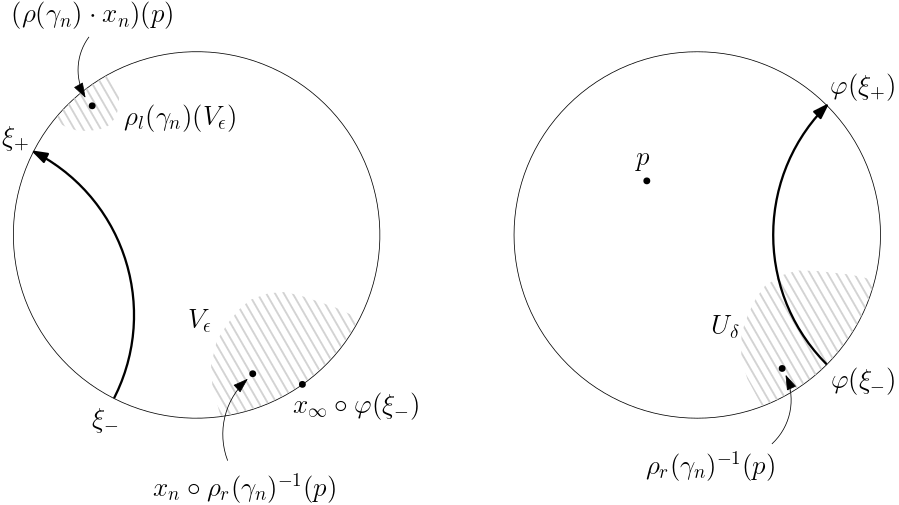
\includegraphics[width=0.7\textwidth]{dynamics.png}
%    \caption{On the proof of Prop \ref{prop:MGH_example}}
%\end{figure}
Now we prove that the MHG constructed in Proposition \ref{prop:MGH_example} are all the MGH spacetime of genus $n$.
\begin{lemma}
    Let $\rho=(\rho_l,\rho_r)$ be a pair of positive Fuchsian representations, and $\varphi :\S \to \S$ be the unique $(\rho_l,\rho_r)$-equivariant orientation-preserving homeomorphism of $\S$. Then $\Lambda(\rho)$ is the unique proper achronal meridian in $\partial \A^{2,1}$ invariant under the action of $\rho(\pi_1(\Sigma_n))$.
\end{lemma}
\begin{proof} 
    Let $\Lambda$ be a proper achronal meridian invariant under the action of $\rho(\pi_1(\Sigma_n))$. We claim $\Lambda \cap \Lambda(\rho)$ is not empty.\\
    Let $\gamma$ be a non-trivial element in $\pi_1(\Sigma_n)$. $\rho_l(\gamma)$ and $\rho_r(\gamma)$ are necessarely hyperbolic elements in $\PSL$, being $\Sigma_n$ compact, and we denote by $\xi^+_l(\gamma)$ and $\xi^+_r(\gamma)$ their attractive fixed points respectively. We have that $\xi^+_r(\gamma) = \varphi(\xi^+_l(\gamma))$, hence
    \[
        (\xi^+_l(\gamma), \xi^+_r(\gamma)) \in \Lambda(\rho).
    \]
    Now, the curve $\Lambda$ must meet the leaf of the left ruling of $\partial \A^{2,1}$
    \[
        \lambda_{\xi^+_r(\gamma)} = \{ (x, \xi^+_r(\gamma)) \ | \ x\in \S \}
    \]
    in a point $(x_0, \xi^+_r(\gamma))$. Then $(\rho_l(\gamma)^k \cdot x_0 ,\xi^+_r(\gamma)) \in \Lambda$ for $k>0$ and, if $x_0\neq \xi^-_l(\gamma)$, passing to the limit on $k$, we have that $(\xi^+_l(\gamma),\xi^+_r(\gamma))$ lies in $\Lambda$.\\
    To conclude assume by contradiction that for every $\gamma \in \pi_1(\Sigma_n)$ the point $(\xi^-_l(\gamma),\xi^+_r(\gamma))$ lies in $\Lambda$. Take $\alpha , \beta \in \pi_1(\Sigma_n)$ so that the axis of $\rho_l(\alpha)$ and $\rho_l(\beta)$ do not intersect. We may assume that the cyclic order of the end points of those axis is
    \begin{equation}\label{eq:order}
        \xi^+_l(\alpha) < \xi^+_l(\beta) < \xi^-_l(\beta) < \xi^-_l(\alpha).
    \end{equation}
    Since $\xi^\pm_r(\alpha) = \varphi(\xi^\pm_l(\alpha))$ and $\xi^\pm_r(\beta) = \varphi(\xi^\pm_l(\beta))$, Equation \ref{eq:order} holds if we replace $\rho_l$ with $\rho_r$.
    On the other hand we assumed that $\Lambda$ contains $(\xi^+_l(\alpha), \xi^-_r(\alpha))$, $(\xi^+_l(\beta), \xi^-_r(\beta))$, $(\xi^-_l(\beta), \xi^+_r(\beta))$, $(\xi^-_l(\alpha), \xi^+_r(\alpha))$. By achronality of $\Lambda$, the cyclic order of the first and second components must be the same, hence
    \[
        \xi^-_l(\alpha) \leq \xi^-_l(\beta) \leq \xi^+_l(\beta) \leq \xi^+_l(\alpha),
    \]
    which contradicts Equation \ref{eq:order}.
\end{proof}
We proved that given a pair $\rho = (\rho_l,\rho_r)$ of positive Fuchsian representations of $\pi_1(\Sigma_n)$ the MGH spacetime $M_\rho := \Omega_\rho / \rho(\pi_1(\Sigma_n))$ is the unique MGH spacetime with holonomy $\rho$.\\
The last step for the classification result is that given a MGH spacetime, the left and right components of the holonomy are necessarely positive Fuchsian.

\begin{observation}\label{rem:bundle}
    By a result of Goldman \cite{goldman1980discontinuous}, a representation $\rho$ is positive Fuchsian if and only if the associated flat $\S$ bundle $E_\rho$, constructed as the quotient of $\widetilde{\Sigma}_n \times \S$ by the diagonal action of $\pi_1(\Sigma_n)$ given by deck transformation on the first factor and by $\rho$ on the second factor, has Euler class $2-2n$. This is also equivalent to the existence of an orientation-preserving fiber bundle isomorphism between $E_\rho$ and the unit tangent bundle of $\Sigma_n$.
\end{observation}
\begin{proposition}
    Let $M$ be an oriented, time-oriented, globally hyperbolic spacetime of genus $n\geq 2$ and let us endow a Cauchy surface $\Sigma$ with the orientation induced by the future normal vector. Then the left and right components of the holonomy $\rho=(\rho_l,\rho_r): \pi_1(\Sigma)\to\PSL\times\PSL$ are positive Fuchsian representations.
\end{proposition}
\begin{proof}
    By Remark \ref{rem:bundle} we have to prove that the $\S$-flat bundles with holonomy $\rho_l$ and $\rho_r$ are isomorphic to the unit tangent bundle. We focus on $\rho_l$, the proof for $\rho_r$ is analogous.\\
    Define $\Phi_l : T^1 \widetilde{\Sigma} \to \widetilde{\Sigma} \times \S$ in the following way: for an element $(x,v) \in T^1 \widetilde{\Sigma}$ let
    \[
        \xi(x,v) = (\xi^l(x,v), \xi^r(x,v)) \in \T
    \]
    be the end-point of the spacelike geodesic ray $exp_x(tv)$ in $\A^{2,1}$, for positive $t$. We define $\Phi_l(x,v)=(x, \xi^l(x,v))$. This map is clearly continuous, proper,
    equivariant and fiber preserving.\\
    To prove that it is bijective it is sufficient to notice that for any $x \in \widetilde{\Sigma}$ the map $\xi_x : T^1_x \widetilde{\Sigma} \to \T$ is an embedding with image the boundary of the totally geodesic plane tangent to $\widetilde{\Sigma}$ at $x$. This boundary is the graph of an orientation-preserving map of $\S$, so the projection $v \to \xi^l(x,v)$ is bijective. Moreover, by the choice of the orientation on $\Sigma$, the orientation on $T^1_x \widetilde{\Sigma}$ corresponds to the orientation induced on $\xi_x (T^1_x \widetilde{\Sigma})$ as graph of an orientation-preserving homeomorphism.
\end{proof}

We conclude this section by stating the classification result. Let the \emph{deformation space} of MGH spacetimes of genus $n$ be:
$$\mathcal{MGH}(\Sigma_n)=\{g\text{ MGH AdS metric on }\Sigma_n\times\R\}/\mathrm{Diff}_0(\Sigma_n\times\R)~,$$
where the group of diffeomorphisms isotopic to the identity acts by pull-back. The holonomy map takes value in the space of representations of $\pi_1(\Sigma_n)$ into $\PSL\times\PSL$ up to conjugation and is well-defined on the quotient $\mathcal{MGH}(\Sigma_n)$.
We proved that the left and right components of the holonomy of elements of $\mathcal{MGH}(\Sigma_n)$ are positive Fuchsian representations, and the space of these representations up to conjugacy is identified with the Teichm\"uller space of $\Sigma_n$
\[
    \mathcal{T}(\Sigma_n)\cong\{\rho:\pi_1(\Sigma_n)\to\PSL\text{ positive Fuchsian representations}\}/\PSL~.
\]
Therefore the holonomy map can be considered as a map 
from $\mathcal{MGH}(\Sigma_n)$ with values in $\mathcal{T}(\Sigma_n)\times\mathcal{T}(\Sigma_n)$.
Hence, we can summarize this section with the following theorem of Mess.

\begin{theorem} \label{thm:classification rgeq2}
The holonomy map $$\rho:\mathcal{MGH}(\Sigma_n)\to\mathcal{T}(\Sigma_n)\times\mathcal{T}(\Sigma_n)$$ is a homeomorphism.
\end{theorem}
